\documentclass[12pt]{exam}
\usepackage[utf8]{inputenc}
\usepackage[a4paper,top=2cm,left=2cm,right=2cm,bottom=2cm]{geometry}
\usepackage{import}
\usepackage[T1]{fontenc}
\usepackage[german,ngerman]{babel}
\usepackage[table]{xcolor}
\usepackage{amsthm, esvect}
\usepackage{mathtools}
\RequirePackage{amssymb, amsfonts, amsmath, latexsym, verbatim, xspace}
\usepackage{systeme}
\usepackage{multicol}
\usepackage{multirow}
\usepackage{framed}
\usepackage{array}
\usepackage{ragged2e}
\usepackage{graphicx}
\usepackage{pdflscape}
\usepackage{epstopdf}
\usepackage{booktabs}
\usepackage{pdfpages}
\usepackage{float} % Allows putting an [H] in \begin{figure} to specify the exact location of the figure
\usepackage{wrapfig} % Allows in-line images such as the example fish picture
\usepackage{tikz, graphicx} % tikz
\usepackage[position=top]{subfig}
\usepackage[bookmarks=true]{hyperref}%Links
\usepackage{enumerate}
\usepackage{enumitem}
\usepackage[german,ruled,vlined,linesnumbered,algosection]{algorithm2e}
\usepackage[labelfont=sf]{caption}
\usepackage{lmodern}
\usepackage{lscape}
\usepackage{tabularx}
\usepackage{systeme}
\usepackage{hhline}
\usepackage{subfiles}
\usepackage{stackengine}
\usepackage{setspace}
\usepackage{MnSymbol}
\usepackage{tcolorbox}
\usepackage{bbm}
\usepackage{url}
\usepackage{xparse}
\usepackage{sectsty}
\usepackage{array}
\usepackage{ragged2e}
\usepackage{listings} %Stellt Code-Snippets sauber dar

% definiert die Sprache
\selectlanguage{German}

% add command for different dates in Swiss fashion
\newcommand{\monthwordlong}[1]{\ifcase#1 \or Januar\or Februar\or März\or April\or Mai\or Juni\or Juli\or August\or September\or Oktober\or November\or Dezember\fi}
\newcommand{\monthwordshort}[1]{\ifcase#1\or Jan\or Feb\or Mar\or Apr\or Mai\or Jun\or Jul\or Aug\or Sept\or Okt\or Nov\or Dez\fi}
\newcommand{\datelong}{\number\day.\:\monthwordlong{\the\month}\:\number\year}
\newcommand{\dateshort}{\number\day.\:\monthwordshort{\the\month}\:\number\year}

% define color of links inside a text
\definecolor{linkblue}{RGB}{0, 0, 80}
\definecolor{plotblue}{RGB}{100, 100, 255}
\definecolor{myblue}{RGB}{8,164,214}
\definecolor{myred}{RGB}{143,42,41}
\definecolor{forestgreen}{RGB}{34,139,34}
\definecolor{highdive}{RGB}{10,169,194}
\definecolor{charcoal}{RGB}{74,74,74}
\hypersetup{
	colorlinks=true,
	linkcolor=linkblue,
	filecolor=magenta,
	urlcolor=plotblue,
	citecolor=linkblue,
	pdfpagemode=FullScreen,
}


\lstdefinestyle{mystyle}{ % definiert den style des Code-Snippets
	%backgroundcolor=\color{backcolour},
	%commentstyle=\color{codegreen},
	%keywordstyle=\color{magenta},
	%numberstyle=\tiny\color{codegray},
	%stringstyle=\color{codepurple},
	basicstyle=\ttfamily\footnotesize,
	breakatwhitespace=false,
	breaklines=true,
	captionpos=b,
	keepspaces=true,
	%numbers=left,
	%numbersep=5pt,
	showspaces=false,
	showstringspaces=false,
	showtabs=false,
	tabsize=4
}
\lstset{style=mystyle}
\qformat{\Large\textbf{Aufgabe \thequestion\hfill\thepoints}}
\newlist{partes}{enumerate}{3}
\setlist[partes]{label=(\alph*)}
\newcommand{\parte}{\item}
\newlist{subpartes}{enumerate}{3}
\setlist[subpartes]{label=\roman*)}
\newcommand{\subparte}{\item}
\setlist[enumerate,1]{%(
	leftmargin=*, itemsep=12pt, label={\textbf{\arabic*.)}}}
\newcommand\answerbox{%%
	\fbox{\rule{2in}{0pt}\rule[-0.1ex]{0pt}{4ex}}}
\pointpoints{Punkt}{Punkte}
\hqword{Frage:}
\hpword{Mögliche Punkte:}
\hsword{Erreicht:}
\htword{Total}
\renewcommand*\half{.5}
\renewcommand{\solutiontitle}{\noindent\textbf{Lösung:}\par\noindent}

% Graphed boxes
\newcommand{\karos}[2]{
  \begin{tikzpicture}
    \draw[step=0.4cm,color=cyan,dotted] (0,0) grid (#1 cm ,#2 cm);
  %  \draw((#1)/2 cm,0)--((#1)/2 cm,/#2)/2cm)
  \end{tikzpicture}
}
\usetikzlibrary{arrows, petri, topaths, graphs}
\linespread{1.2} % Line spacing

%=========================================================
\newenvironment{parcols}[1][]{
    \begin{parts}\begin{multicols}{#1}
}{
    \end{multicols}\end{parts}
}
%=========================================================
\newenvironment{itemcols}[1][]{
	\begin{itemize}\begin{multicols}{#1}
		}{
	\end{multicols}\end{itemize}
}

%=========================================================
\newcommand{\antwort}[1]{
	{\setlength{\textwidth}{\textwidth}\fillwithgrid{#1cm}\vspace{5pt}}
}

%=========================================================
% Karriertes Papier für Antwort MIT OVERLAY
\tcbuselibrary{breakable,skins}
\usetikzlibrary{mindmap,trees}
\newlength\tindent
\setlength{\tindent}{\parindent}
\setlength{\parindent}{0pt}
\setlength{\parskip}{0pt}

\newtcolorbox{gridspace}[1]{%
	enhanced,
	breakable,
	blanker,
	boxrule=0pt,
	left=5mm,
	right=5mm,
	top=5.75mm,
	bottom=0mm,
	boxsep=0pt,
	height=#1cm,
	width=16cm,
	before upper={
		\begingroup
		\setlength{\baselineskip}{5.75mm}
		\setlength{\parskip}{0pt}
		\setlength{\lineskip}{0pt}
		% keep every paragraph on the grid rhythm
		%\everypar{\vspace{0pt}\strut}
		% math formulas shifted by one grid row
		\let\oldbracketopen\[
		\renewcommand{\[}{\vspace{-5mm}\oldbracketopen}
		% Align displayed formulas to the grid
		\setlength{\abovedisplayskip}{0pt}
		\setlength{\belowdisplayskip}{0pt}
		\setlength{\abovedisplayshortskip}{0pt}
		\setlength{\belowdisplayshortskip}{0pt}
		% Enumerate follows the same rhythm
		\setlist[enumerate]{leftmargin=6mm,itemsep=0mm,topsep=0pt,parsep=0pt,partopsep=0pt}
		\setlist[itemize]{leftmargin=6mm,itemsep=10mm,topsep=0pt,parsep=0pt,partopsep=0pt}},
	after upper={
		\endgroup},
	underlay={
		\draw[step=5mm,color=gray!55] (interior.south west) grid (interior.north east);}
}

%%
% Math Arrows
%%
\newcommand{\same}{\ensuremath{\Longleftrightarrow}}
\renewcommand{\to}{\ensuremath{\longrightarrow}}
\newcommand{\qsame}{\quad\same\quad}
\newcommand{\dsame}{\ensuremath{:\Leftrightarrow}}
\newcommand{\qdsame}{\quad\dsame\quad}
\newcommand{\ldsame}{\ensuremath{:\Longleftrightarrow}}
\newcommand{\samedef}{\ensuremath{\us {\text{def}} \Leftrightarrow}}
\newcommand{\qsamedef}{\quad\samedef\quad}
\newcommand{\lsamedef}{\ensuremath{\us {\text{def}} \Longleftrightarrow}}
\newcommand{\qlsamedef}{\quad\lsamedef\quad}


%%
% Mengendefinitionen
%%
\newcommand{\M}{\ensuremath{\mathcal{M}}}
\newcommand{\N}{\ensuremath{\mathbb{N}}}
\newcommand{\Z}{\ensuremath{\mathbb{Z}}}
\newcommand{\Q}{\ensuremath{\mathbb{Q}}}
\newcommand{\I}{\ensuremath{\mathbb{I}}}
\newcommand{\R}{\ensuremath{\mathbb{R}}}
\newcommand{\C}{\ensuremath{\mathbb{C}}}
\renewcommand{\S}{\ensuremath{\mathbb{S}}}
\newcommand{\Prim}{\ensuremath{\mathbb{P}}}
\newcommand{\0}{\ensuremath{\emptyset}}
\renewcommand{\Re}{\ensuremath{\operatorname{Re}}}
\renewcommand{\Im}{\ensuremath{\operatorname{Im}}}
\newcommand{\strich}{\ensuremath{\big\vert}}

%%
% Mengenoperation
%%
\renewcommand{\nin}{\not\in}


%%
% Logisches Und und Oder
%%
\newcommand{\sand}{\ensuremath{\; \land \;}}
\newcommand{\sor}{\ensuremath{\; \lor \;}}
\renewcommand{\*}{\ensuremath{\cdot}}
\newcommand{\oder}{\vee}
\newcommand{\n}{\neg}
\newcommand{\und}{\wedge}


%%
% Bei Integral, Summe,... die Grenzen über bzw.
% unter das Zeichen
%%
\renewcommand{\d}[1]{\ensuremath{\operatorname{d}\!{#1}}}
\newcommand{\Sum}{\sum\limits}
\newcommand{\Prod}{\prod\limits}
\newcommand{\Min}{\min\limits}
\newcommand{\Max}{\max\limits}
\newcommand{\Lim}{\lim\limits}
\newcommand{\Inf}{\inf\limits}
\newcommand{\Sup}{\sup\limits}
\newcommand{\Liminf}{\liminf\limits}
\newcommand{\Limsup}{\limsup\limits}
%\renewcommand{\Cup}{\bigcup\limits}
%\renewcommand{\Cap}{\bigcap\limits}
\newcommand{\Otimes}{\bigotimes\limits}
\newcommand{\Oplus}{\bigoplus\limits}


%%
% Arcus Cotangens, Logarithmus
%%
\let\oldsin\sin
\renewcommand{\sin}[1]{\oldsin{\left(#1\right)}}
\let\oldcos\cos
\renewcommand{\cos}[1]{\oldcos{\left(#1\right)}}
\let\oldtan\tan
\renewcommand{\tan}[1]{\oldtan{\left(#1\right)}}
\let\oldarcsin\arcsin
\renewcommand{\arcsin}[1]{\oldarcsin{\left(#1\right)}}
\let\oldarccos\arccos
\renewcommand{\arccos}[1]{\oldarccos{\left(#1\right)}}
\let\oldarctan\arctan
\renewcommand{\arctan}[1]{\oldarctan{\left(#1\right)}}
\let\oldln\ln
\renewcommand{\ln}[1]{\oldln{\left(#1\right)}}
\newcommand{\Log}[2]{\ensuremath{\operatorname{log}_{#1}\left(#2\right)}}
\newcommand{\e}{\operatorname{e}}
\renewcommand{\exp}[1]{\ensuremath{\operatorname{\e}^{#1}}}


%%
% Griechische Buchstaben
%%
\renewcommand{\epsilon}{\ensuremath{\varepsilon}}
\renewcommand{\phi}{\varphi}
\renewcommand{\l}{\lambda}
\renewcommand{\t}{\tau}


%%
% Bezeichnungen
%%
\newcommand{\Rgn}{\R_{>0}} % R grösser Null
\newcommand{\Rad}{\operatorname{Rad}}   % Radikal
\newcommand{\kgV}{\operatorname{kgV}}   % Kleinster gemeinsame Vielfache
\newcommand{\ggT}{\operatorname{ggT}}   % Grösster gemeinsame Teiler
\newcommand{\winkel}{\sphericalangle}          % Winkelsymbol
\DeclarePairedDelimiter\abs{\lvert}{\rvert} % besserer Betrag
\makeatletter
\let\oldabs\abs
\def\abs{\@ifstar{\oldabs}{\oldabs*}}
\makeatother


%%
% Vektorgeometrie
%%
\renewcommand{\v}[1]{\vv{#1}}       % besserer Pfeil über Buchstaben
\renewcommand{\vec}[2]{\begingroup\renewcommand{\arraystretch}{1}\left(\begin{array}{c} #1 \\ #2 \end{array}\right)\endgroup}   % two dimensional vector
\renewcommand{\Vec}[3]{\begingroup\renewcommand{\arraystretch}{1}\left(\begin{array}{c} #1 \\ #2 \\ #3 \end{array}\right)\endgroup}      % three dimensional vector


%%
% Text
%%
\newcommand*{\Ueq}[1]{\mathrel{\mathop{=}\limits_{\text{#1}}}}
\newcommand*{\Oeq}[1]{\mathrel{\stackrel{\text{#1}}{=}}}
\newcommand{\utext}[2]{\underbrace{#1}_{\substack{#2}}}
\newcommand{\otext}[2]{$\overbrace{\textrm{#1}}^{\textrm{#2}}$}
\newcommand{\lineortext}[1]{\hspace{0,1cm}\underline{\hspace{0.1cm}\hphantom{#1}\hspace{0.1cm}}\hspace{0,1cm}} % Lückentext erstellen
\newcommand{\gap}[1]{\rule{#1 cm}{1pt}}
\pagestyle{headandfoot}
\firstpageheader{}{}{}
\runningheader{\date}{}{\themeshort}
\runningheadrule
\firstpagefooter{}{}{}
\runningfooter{}{Viel Erfolg!}{Seite \thepage\:von \numpages}
\runningfootrule
%\printanswers % falls kommentiert werden die Antwortenfelder angezeigt
\graphicspath{{Analysis/data-analysis/},{Algebra/data-algebra/},{Geometrie/data-geometrie/}}
%=========================================================
\newcommand{\theme}{Zwischenprüfung 2025}
\newcommand{\themeshort}{GZP 2025}
\renewcommand{\date}{27.05.25}
%=========================================================
\begin{document}
\fontsize{14}{14}\selectfont
%=========================================================
%------------------- TEIL EINS
%=========================================================
\noindent
\begin{tabular*}{\textwidth}{l @{\extracolsep{\fill}}l @{\extracolsep{7pt}}l}
     Kanton St. Gallen & & \multirow{4}{4em}{
\includegraphics[scale=0.2]{../Header/wappen_sg.png}}\\
     Bildungsdepartement & & \\
     & & \\
     \textbf{Kantonsschule Heerbrugg} & & \\
\end{tabular*}
\vspace{1cm}\newline
%--------------------
\begingroup
\renewcommand{\arraystretch}{1.5}
\begin{tabular*}{\textwidth}{l @{\extracolsep{\fill}}l @{\extracolsep{6pt}}l}\hline
    {\bf \theme} & {\bf Lehrpersonen:} & Dc, Fh, Gt, Gu, Ss \\\hline
    {\bf Mathematik, Teil 1 (ohne TR)} & {\bf Dauer:} & 45 Minuten \\\hline
    {\bf Name:} & {\bf Klasse:} &  \\\hline
    {\bf Vorname:} & {\bf Note:} & \\\hline
\end{tabular*}
\endgroup
\begin{center}
    \textbf{Bewertungstabelle}\\
    {\small Wird von der Lehrperson ausgefüllt}\\
    \vspace{10pt}
    \addpoints
    \partialgradetable{ersterTeil}[h][questions]\\[0.25in]
    \partialgradetable{zweiterTeil}[h][questions]\\[1cm]
    Der Rechenweg muss \textbf{vollständig und nachvollziehbar} sein. \\
    Unvollständige Lösungswege haben einen Punktabzug zur Folge.\\
    Es sind keine Hilfsmittel zugelassen.\\
\end{center}
\rule[1ex]{\textwidth}{1pt}


\newpage
\begin{questions}
\begingradingrange{ersterTeil} % unterteilt die Notentabelle in zwei Teile
%=========================================================
%----------------------------TESTFRAGEN
%=========================================================
\question[3]
Berechne die Lösungsmenge der folgenden Gleichungen für $x$.
\begin{parcols}[2]
	\part $2x^2+3=7x$
	\part $11-6(x-14)=20-3(2x-25)$
\end{parcols}
\ifthenelse{\boolean{printanswers}}
{\begin{solution}
		\begin{parts}
			\part \begin{align*}
				2x^2+3&=7x \\
				2x^2-7x+3&=0\\
				x_{1,2}&=\frac{-(-7)\pm\sqrt{(-7)^2-4\*2\*3}}{2\*2}\Rightarrow\mathbb{L}=\left\{\frac{1}{2},3\right\}
			\end{align*}
			\part \begin{align*}
				11-6x+84&=20-6x+75\\
				-6x+95&=-6x+95\Rightarrow\mathbb{L}=\R
			\end{align*}
		\end{parts}
\end{solution}}
{\vspace{5pt}\antwort{9}\vfill}

\question[2]
Vereinfache den nachfolgenden Term so weit wie möglich. Im Endergebnis sollen keine negativen Exponenten vorhanden sein.
\[\frac{x\*x^4\left(y^{-2}\*\sqrt{y^{16}}\right)}{x^{-2}\*x^7\*\sqrt{x^4}}\]
\ifthenelse{\boolean{printanswers}}
{\begin{solution}
	\[\frac{x\*x^4\left(y^{-2}\*\sqrt{y^{16}}\right)}{x^{-2}\*x^7\*\sqrt{x^4}}=x^5\*y^{-2}\*y^8\*x^{-5}\*x^{-2}=y^6\*x^{-2}=\frac{y^6}{x^2}\]
\end{solution}}
{\vspace{5pt}\antwort{9}\newpage}


%------------------------------------------------
\question[3]
Entscheide in der Tabelle unten, ob die Gleichungen richtig oder falsch sind. Die Antworten müssen nicht begründet werden.\newline
\begin{small}
	Bewertung: Für $0-2$ korrekte Antworten gibt es keine Punkte; $3$ korrekte Antworten $1.5$ Punkt und falls alle Antworten korrekt sind, gibt es $3$ Punkte.
\end{small}
\ifthenelse{\boolean{printanswers}}
{\begin{solution}
	\begin{table}[H]
		\centering
		\begin{tabular}{|p{10cm}|c|c|}\hline
			& richtig & falsch \\\hline
			\[\frac{b}{a}+\frac{a}{b}=1\] & & {\bf X} \\\hline
			\[\frac{1}{\sqrt{x}}+\frac{1}{\sqrt{y}}=\frac{\sqrt{x}+\sqrt{y}}{\sqrt{xy}}\] & {\bf X} & \\\hline
			\[\left(\frac{a^n}{a^{-n}}\right)^2\*a^{2n}=a^{4n^2+2n}\] & {\bf X} & \\\hline
			\[\frac{\frac{x+y}{x}}{\frac{y}{x-y}}=\frac{x^2-2xy-y^2}{xy}\] & & {\bf X} \\\hline
		\end{tabular}
	\end{table}
\end{solution}}
{\begin{table}[H]
		\centering
		\begin{tabular}{|p{10cm}|c|c|}\hline
			& richtig & falsch \\\hline
			\[\frac{b}{a}+\frac{a}{b}=1\] & & \\\hline
			\[\frac{1}{\sqrt{x}}+\frac{1}{\sqrt{y}}=\frac{\sqrt{x}+\sqrt{y}}{\sqrt{xy}}\] & & \\\hline
			\[\left(\frac{a^n}{a^{-n}}\right)^2\*a^{2n}=a^{4n^2+2n}\] & & \\\hline
			\[\frac{\frac{x+y}{x}}{\frac{y}{x-y}}=\frac{x^2-2xy-y^2}{xy}\] & & \\\hline
		\end{tabular}
	\end{table}
	\antwort{13.5}\newpage}

%------------------------------------------------
\question[4]
Berechne die fehlenden Grössen $w, x, y$ und $z$.
\begin{figure}[H]
	\centering
	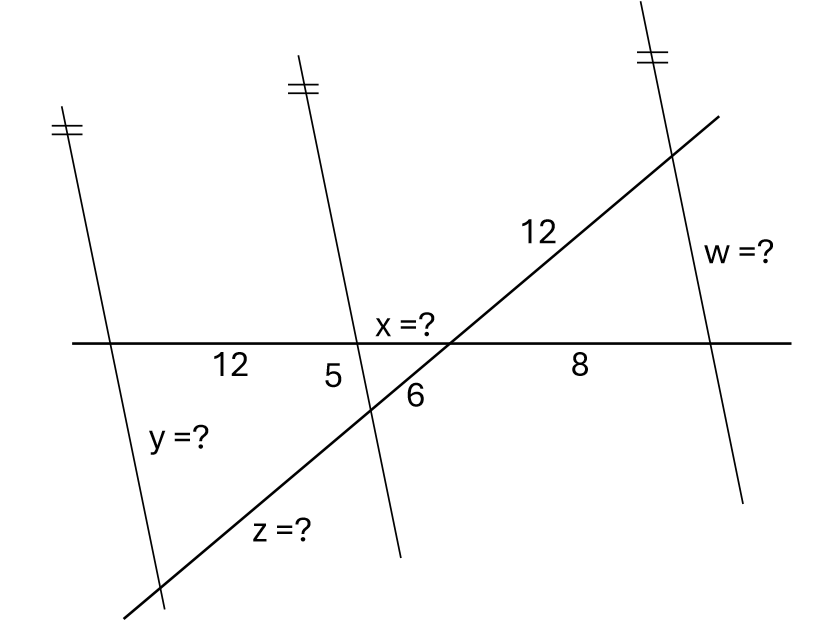
\includegraphics[scale=0.4]{Geometrie/data-geometrie/GZP25_Teil1Aufg4.png}
\end{figure}
\ifthenelse{\boolean{printanswers}}
{\begin{solution}
		\begin{table}[H]
			\centering
			\begin{tabular}{p{6cm} p{6cm}}
				\[\frac{w}{12}=\frac{5}{6}\quad\Rightarrow w=10\] &	\[\frac{x}{16}=\frac{8}{12}\quad\Rightarrow x=4\] \\
				\[\frac{y}{x+12}=\frac{5}{x}\quad\Rightarrow y=20\] & \[\frac{z}{6}=\frac{12}{x}\quad\Rightarrow z=18\]
			\end{tabular}
		\end{table}
\end{solution}}
{\antwort{17}\newpage}


%------------------------------------------------
\question[3]
Berechne die Lösungsmenge der folgenden Gleichung für $x$.
\[\frac{x-1}{x+3}-\frac{x-4}{x+5}=\frac{7x+13}{x^2+8x+15}\]
\ifthenelse{\boolean{printanswers}}
{\begin{solution}
		Zuerst untersuchen wir den Hauptnenner: $(x+3)(x+5)$. Das bedeutet die Definitionsmenge dieser Gleichung ist: \[\Rightarrow D=\R\setminus\left\{-3,-5\right\}.\] Lasst uns als nächstes die Gleichung lösen:
		\begin{align*}
			\frac{(x-1)(x+5)}{(x+3)(x+5)}-\frac{(x-4)(x+3)}{(x+3)(x+5)}&=\frac{7x+13}{(x+3)(x+5)} &&\vert\*(x+3)(x+5)\\
			(x^2+4x-5)-(x^2-x-12)&=7x+13 &&\vert TU\\
			5x+7&=7x+13&& \vert-5x-13\\
			-6&=2x &&\vert\div 2\\
			x&=-3 \qquad\Rightarrow \mathbb{L}=\emptyset
		\end{align*}
\end{solution}}
{\antwort{22}\newpage}


%------------------------------------------------
\question[7]\
\begin{figure}[H]
	\centering
	\begin{tikzpicture}[cross/.style={draw, cross out, minimum size=2*(#1-1pt), inner sep=0pt, outer sep=0pt}, x=10mm, y=10mm,
		>=latex,   %Voreinstellung für Pfeilspitzen
		font= \footnotesize, scale=0.9]
		%Raster zeichnen
		\draw [color=gray!50]  [step=10mm] (-2.2,-2.2) grid (9.7,6.7);
		% Achsen zeichnen
		\draw[->,thick] (-2.4,0) -- (9.9,0) node[below] {\normalsize $x$};
		\draw[->,thick] (0,-2.4) -- (0,6.9) node[left] {\normalsize $y$};
		% Achsen beschriften
		\foreach \x in {-2,-1,1,2,...,9} \draw (\x,-.1) -- (\x,.1) node[below=4pt] {$\x$};
		\foreach \y in {-2,-1,1,2,...,6} \draw (-.1,\y) -- (.1,\y) node[left=4pt] {$\y$};
		% Besserer Ursprung
		\draw[color=black] (0pt,-7pt) node[right] {$0$};
		%Funktionen zeichnen:
		\clip(-2.2,-2.2) rectangle (9.2,6.7); %Bildbereich
		\draw[black,domain=-2:9,samples=100,line width=1.5pt] plot (\x, {-5/4*\x+19/4});
		\draw[color=plotblue, fill=plotblue] (-1,6) circle (2.5pt);
		\draw[color=plotblue, fill=plotblue] (3,1) circle (2.5pt);
		\draw[color=plotblue] (-1.3,5.7) node {\normalsize $A$};
		\draw[color=plotblue] (3.3,1.2) node {\normalsize $B$};
		\draw[color=black] (5.2,-1.3) node {\normalsize $f$};
		\ifthenelse{\boolean{printanswers}}{
		\draw[forestgreen,domain=-2:9,samples=100,line width=1.5pt] plot (\x, {2*\x-1});
		\draw[color=forestgreen] (3.2,4.6) node {\normalsize $g$};}{}
	\end{tikzpicture}
\end{figure}
\begin{parts}
	\part Gib die Funktionsgleichung der dargestellten Gerade $f$ an.
	\part Zeichne die Gerade $g:y=2x-1$ ins Koordinatensystem ein.
	\part Bestimme die Gleichung der zu $g$ senkrechten Gerade $h$, die durch den Punkt $P(5,-7)$ geht.
	\part Bestimme den Schnittpunkt der beiden Geraden $f$ und $g$.
\end{parts}
\ifthenelse{\boolean{printanswers}}
{\begin{solution}
		\begin{parts}
			\part $f:y=mx+q$ durch die beiden Punkte $A(-1,6)$ und $B(3,1)$. Für die Steigung gilt: \[m_f=\frac{1-6}{3-(-1)}=-\frac{5}{4}.\] Wir können den einen oder anderen Punkt einsetzen, um den $y-$ Achsenabschnitt zu berechnen:
			\begin{align*}
				6&=-\frac{5}{4}\*(-1)+q &&1=-\frac{5}{4}\*3+q\\
				&\Rightarrow q=\frac{19}{4}\\
				&\Rightarrow f:y=-\frac{5}{4}x+\frac{19}{4}
			\end{align*}
			\part Im Koordinatensystem eingezeichnet
			\part Da die Gerade senkrecht zu $g$ steht, gilt: $m_h=-\frac{1}{m_g}=-\frac{1}{2}$. Der Punkt $P(5,-7)$ gehört zum Graphen:
			\begin{align*}
				-7&=-\frac{1}{2}\*5+q\\
				q&=-7+\frac{5}{2}=-\frac{9}{2}.\\
				&\Rightarrow h:y=-\frac{1}{2}x-\frac{9}{2}
			\end{align*}
			\part Setze die beiden Funktionsgleichungen von $f$ und $g$ gleich:
			\begin{align*}
				-\frac{5}{4}x+\frac{19}{4}&=2x-1 &&\vert \*4\\
				-5x+19&=8x-4\\
				23&=13x\\
				x&=\frac{23}{13}\\
				&\ \\
				y&=2\*\frac{23}{13}-1=\frac{46}{13}-\frac{13}{13}=\frac{33}{13}\\
				&\Rightarrow S\left(\frac{23}{13},\frac{33}{13}\right)
			\end{align*}
		\end{parts}
\end{solution}}
{\vspace{5pt}\antwort{11.5}\newpage\antwort{25}\newpage}

%------------------------------------------------
\question[3]
Entscheide in der Tabelle unten, ob die Gleichungen richtig oder falsch sind. Die Antworten müssen nicht begründet werden.\newline
\begin{small}
	Bewertung: Für $0-2$ korrekte Antworten gibt es keine Punkte; $3$ korrekte Antworten $1.5$ Punkt und falls alle Antworten korrekt sind, gibt es $3$ Punkte.\newline
\end{small}
\ifthenelse{\boolean{printanswers}}
{\begin{solution}
		\begingroup
		\renewcommand{\arraystretch}{1.5}
		\begin{table}[H]
			\centering
			\begin{tabular}{|p{6cm}|c|c|}\hline
				& richtig & falsch \\\hline
				$\displaystyle\tan{125^\circ}<0$ & {\bf X} & \\\hline
				$\displaystyle\sin{\alpha}=\sin{180^\circ-\alpha}$ & {\bf X} & \\\hline
				$\displaystyle\cos{34^\circ}=\cos{200^\circ}$ & & {\bf X} \\\hline
				$\displaystyle\cos{10^\circ}\*\tan{10^\circ}=\sin{10^\circ}$ & {\bf X} & \\\hline
			\end{tabular}
		\end{table}
		\endgroup
\end{solution}}
{\begin{minipage}{0.35\linewidth}
		\centering
		\begin{tikzpicture}[cross/.style={draw, cross out, minimum size=2*(#1-1pt), inner sep=0pt, outer sep=0pt}, x=10mm, y=10mm,
			>=latex,   %Voreinstellung für Pfeilspitzen
			font= \footnotesize, scale=2.4]
			%Raster zeichnen
			% \draw [color=gray!50]  [step=5mm] (-1.1,-1.1) grid (1.1,1.1);
			% Achsen zeichnen
			\draw[->,thick] (-1.1,0) -- (1.3,0) node[right, below] {\normalsize $x$};
			\draw[->,thick] (0,-1.1) -- (0,1.3) node[above, left] {\normalsize $y$};
			% Achsen beschriften
			\foreach \x in {-1,1} \draw (\x,-.03) -- (\x,.03);
			\foreach \y in {-1,1} \draw (-.03,\y) -- (.03,\y);
			\draw[color=black] (1.05,-.1) node {$1$};
			\draw[color=black] (-.05,1.1) node {$1$};
			\draw[color=black] (-1.1,-.1) node {$-1$};
			\draw[color=black] (-.1,-1.1) node {$-1$};
			% Besserer Ursprung
			\draw[color=black] (0pt,-3pt) node[right] {$0$};
			% Funktionen zeichnen:
			\clip(-1.1,-1.1) rectangle (1.1,1.1); %Bildbereich
			\draw circle [radius=1];
		\end{tikzpicture}
	\end{minipage}
	\hfill
	\begin{minipage}{0.6\linewidth}\begingroup
	\renewcommand{\arraystretch}{1.5}
	\begin{table}[H]
		\centering
		\begin{tabular}{|p{6cm}|c|c|}\hline
			& richtig & falsch \\\hline
			$\displaystyle\tan{125^\circ}<0$ & & \\\hline
			$\displaystyle\sin{\alpha}=\sin{180^\circ-\alpha}$ & & \\\hline
			$\displaystyle\cos{34^\circ}=\cos{200^\circ}$ & & \\\hline
			$\displaystyle\cos{10^\circ}\*\tan{10^\circ}=\sin{10^\circ}$ & & \\\hline
		\end{tabular}
	\end{table}
	\endgroup
\end{minipage}}
\question[3]
\begin{minipage}{0.3\linewidth}
	\begin{parts}
		\part Bestimme $\displaystyle\frac{A_2}{A_1}$
		\part Bestimme $\displaystyle\frac{A_3}{A_1}$
	\end{parts}
\end{minipage}
\hfill
\begin{minipage}{0.65\linewidth}
	\centering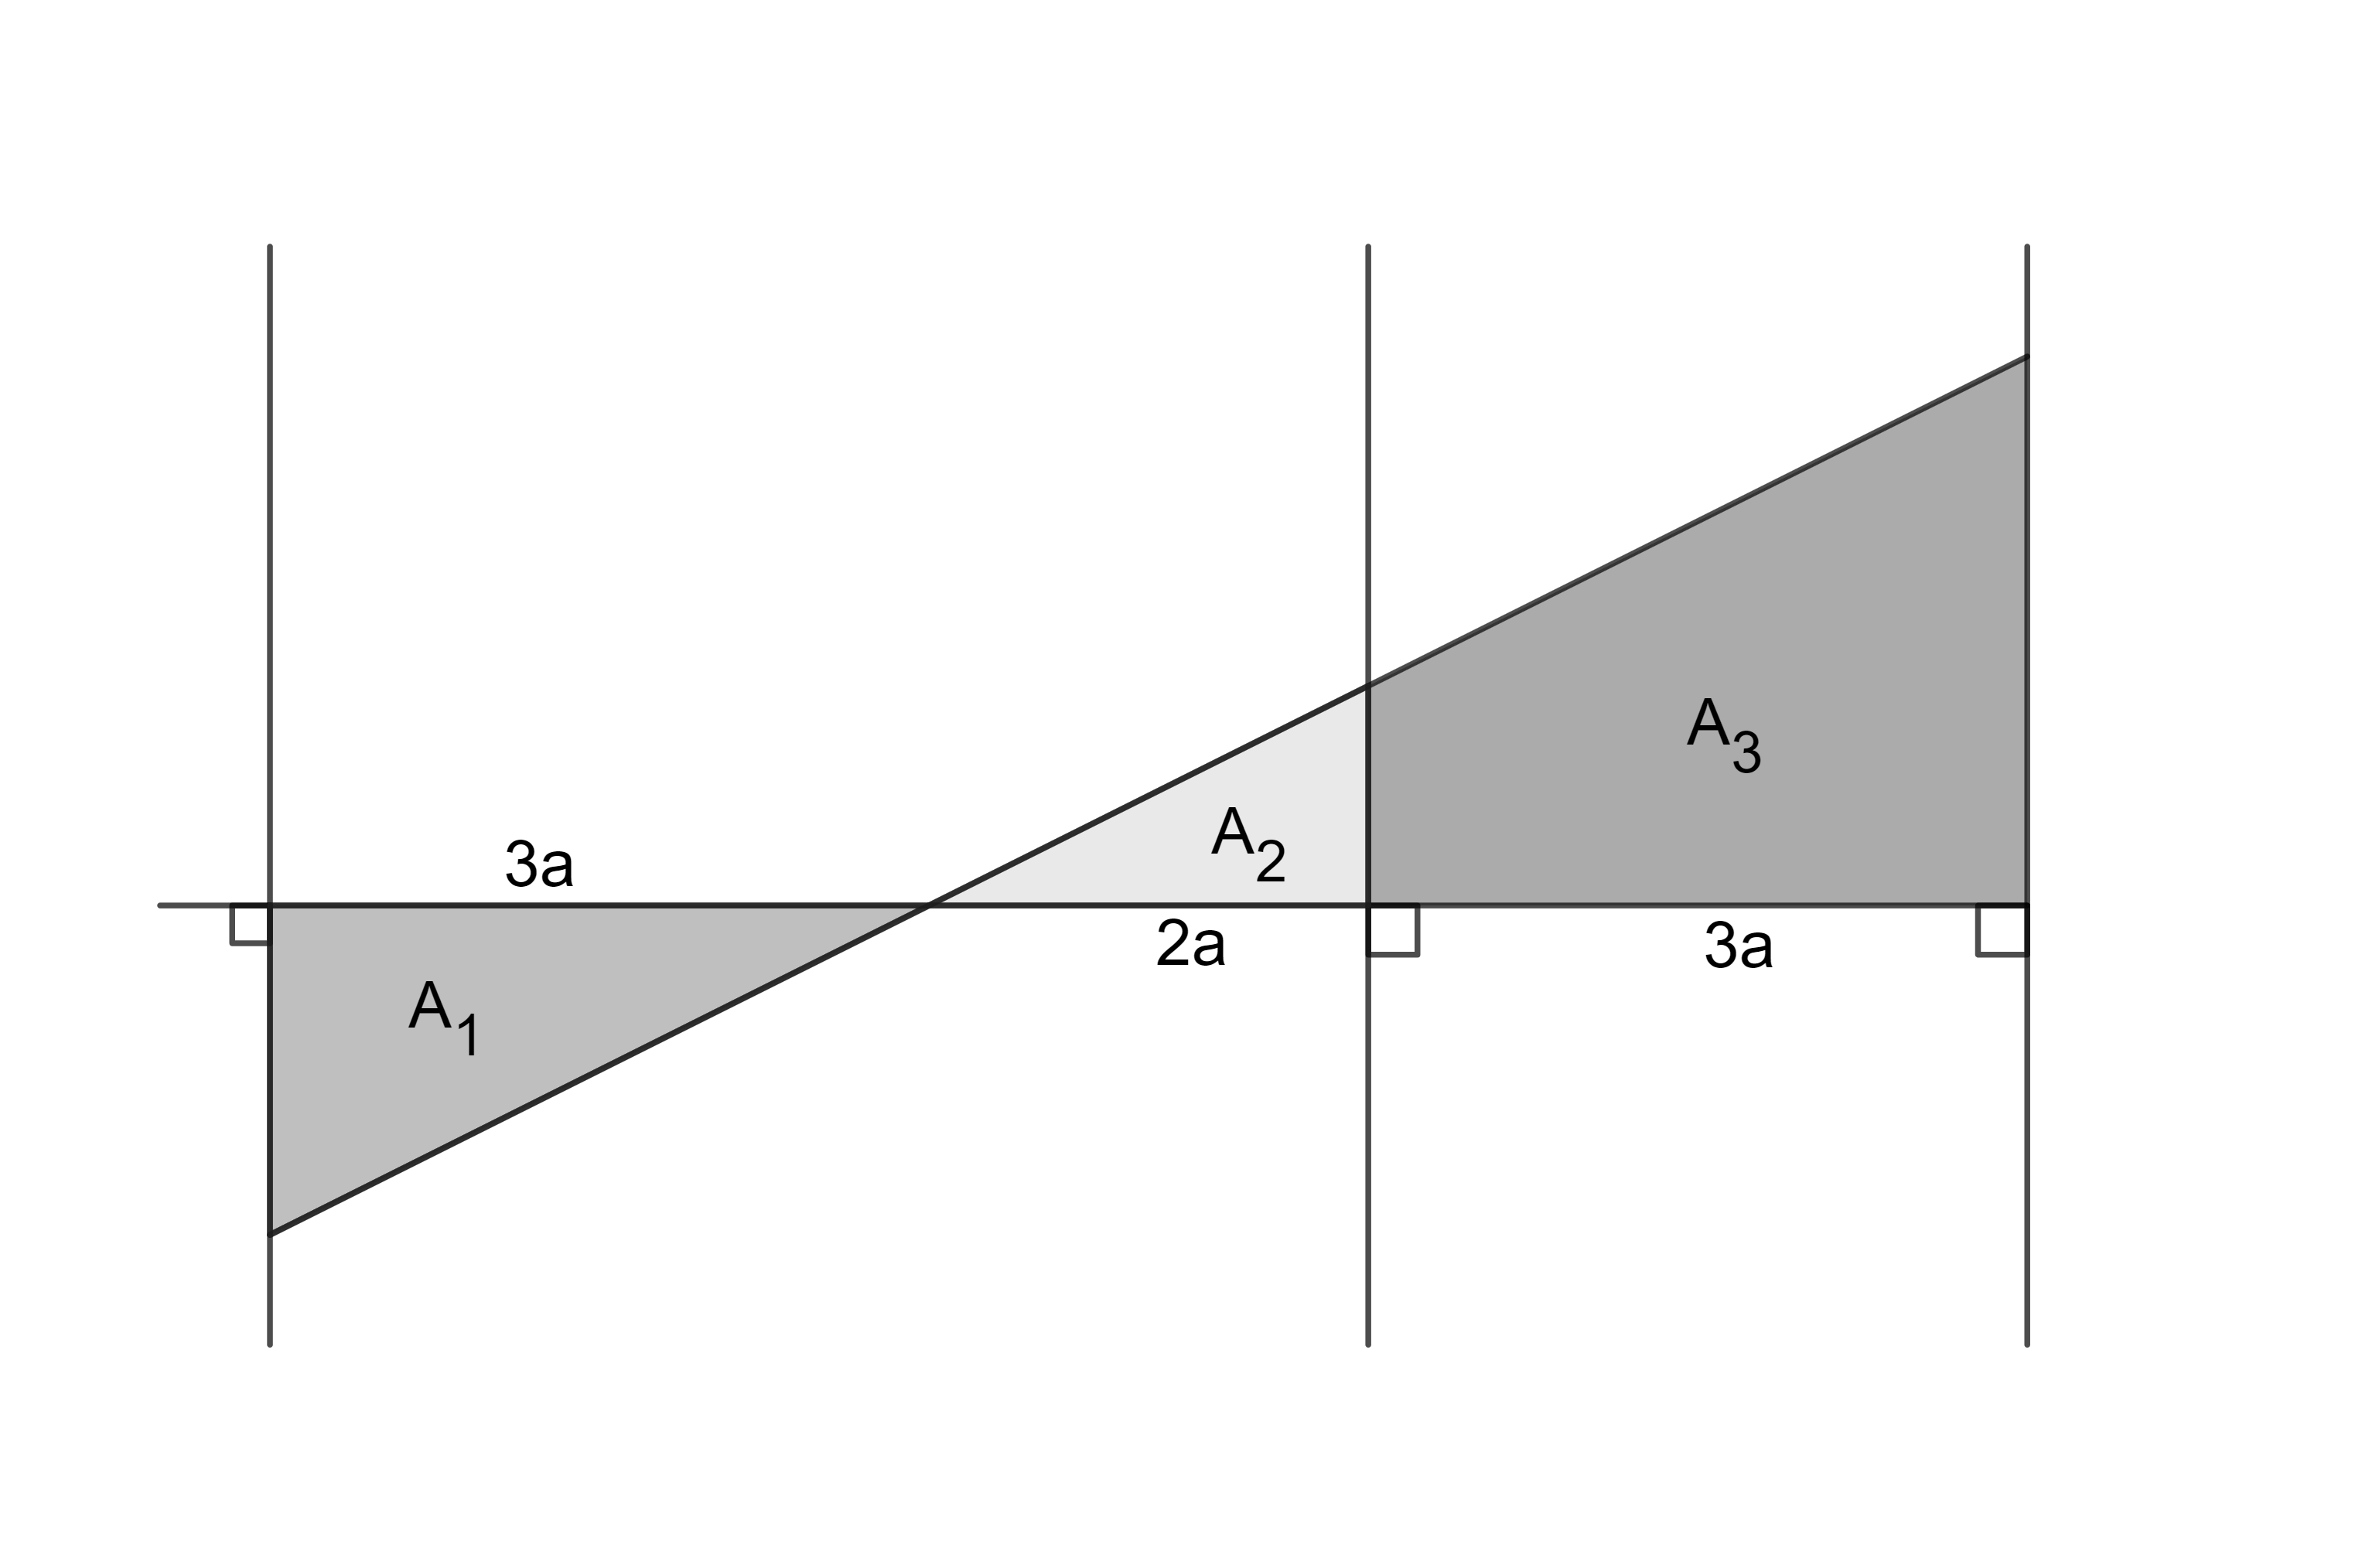
\includegraphics[scale=0.22]{Geometrie/data-geometrie/GZP25_Teil1Aufg5.png}
\end{minipage}
\ifthenelse{\boolean{printanswers}}
{\begin{solution}
	\begin{parts}
		\part\begin{align*}
			\frac{A_2}{A_1}&=\left(\frac{2a}{3a}\right)^2=\frac{4}{9}\\
			A_2&=\frac{4}{9}A_1\\
		\end{align*}
		\part\begin{align*}
			\frac{A_2+A_3}{A_1}&=\left(\frac{5a}{3a}\right)^2=\frac{25}{9}\\
			A_2+A_3&=\frac{25}{9}A_1\\
			\Rightarrow A_3+\frac{4}{9}A_1&=\frac{25}{9}A_1=\left(\frac{25}{9}-\frac{4}{9}\right)\*A_1=\frac{7}{3}A_1\\
			\frac{A_3}{A_1}&=\frac{7}{3}
		\end{align*}
	\end{parts}
\end{solution}}
{\vspace{7pt}\antwort{9.5}\newpage}


%------------------------------------------------
\question[4]
Löse das Gleichungssystem ohne Diskussion der Sonderfälle.
\[\systeme[xy]{a\*x+2y=4,x+y=a}\]
\ifthenelse{\boolean{printanswers}}
{\begin{solution}
		\begin{align*}
			&\systeme[xy]{a\*x+2y=4,-2x-2y=-2a}\\
			ax-2x&=4-2a\\
			x(a-2)&=-2(a-2)\\
			x&=\frac{-2(a-2)}{(a-2)}=-2\\
			&\Rightarrow y=a+2 \qquad\Rightarrow \mathbb{L}=\left\{(-2,a+2)\right\}
		\end{align*}
\end{solution}}
{\antwort{22}}

\ifthenelse{\boolean{printanswers}}
{}{{\bf Reserve:}\newline\antwort{24.5}\newpage {\bf Reserve:}\newline\antwort{24.5}}

\endgradingrange{ersterTeil} % beendet die Unterteilung der Notentabelle
\end{questions}
%=========================================================
%------------------- TEIL ZWEI
%=========================================================
\newpage
\thispagestyle{empty}
\noindent
\begin{tabular*}{\textwidth}{l @{\extracolsep{\fill}}l @{\extracolsep{7pt}}l}
     Kanton St. Gallen & & \multirow{4}{4em}{
\includegraphics[scale=0.2]{../Header/wappen_sg.png}}\\
     Bildungsdepartement & & \\
     & & \\
     \textbf{Kantonsschule Heerbrugg} & & \\
\end{tabular*}
\vspace{1cm}\newline
\begingroup
\renewcommand{\arraystretch}{1.5}
\begin{tabular*}{\textwidth}{l @{\extracolsep{\fill}}l @{\extracolsep{6pt}}l}\hline
    \textbf{\theme} & {\bf Lehrpersonen:} & Dc, Fh, Gt, Gu, Ss \\\hline
    \textbf{Mathematik, Teil 2 (mit TR)} & {\bf Dauer:} & 45 Minuten \\\hline
    \textbf{Name:} & {\bf Klasse:} &  \\\hline
    \textbf{Vorname:} &  & \\\hline
\end{tabular*}
\endgroup

\begin{center}
    \textbf{Bewertungstabelle}\\
    {\small Wird von der Lehrperson ausgefüllt}\\
    \vspace{10pt}
    \addpoints
    \partialgradetable{zweiterTeil}[h][questions]\\[1cm]
    Der Rechenweg muss \textbf{vollständig und nachvollziehbar} sein. \\
    Unvollständige Lösungswege haben einen Punktabzug zur Folge.\\
    Als Hilfsmittel ist ein Taschenrechner (TI-Nspire CX-CAS) erlaubt.\\
\end{center}

\noindent
\rule[1ex]{\textwidth}{1pt}

\vfill
\begin{center}
    %\Huge{Repetitionsprüfung}
\end{center}
%========================================================
\newpage
\begin{questions}
\setcounter{question}{9} % fixiert den counter für fortlaufende Nummerierung
\begingradingrange{zweiterTeil} % beginnt die Unterteilung der Notentabelle
%=========================================================
%-------------------TESTFRAGEN
%=========================================================
\question[3]
\begin{parts}
	\part Bestimme die Gleichung $f:y=ax^2+bx+c$ einer quadratischen Funktion mit den Nullstellen (zeros) $x_1=2$ und $x_2=4$ so, dass die Parabel durch den Punkt $P(-1 \vert 30)$ geht.
	\part Gib die Koordinaten des Scheitelpunktes (vertex) an.
\end{parts}
\ifthenelse{\boolean{printanswers}}
{\begin{solution}
		\begin{parts}
			\part \begin{enumerate}
				\item Mit Hilfe der Nullstellenform: $f(x)=a\*(x-2)(x-4)$. Da der Punkt P zur Parabel gehört gilt: \[30=a\*(-1-2)(-1-4) \Rightarrow a=2.\] Also folgt: \[f(x)=2(x-2)(x-4)=2x^2-12x+16\]
				\item Mit Hilfe eines Gleichungssystems: Da die Punkte $N_1(2,0), N_2(4,0)$ und $P(-1,30)$ zur Parabel gehören, folgt \[\left\{\begin{array}{l}a\*2^2+b\*2+c=0\\a\*4^2+b\*4+c=0\\a\*(-1)^2+b\*(-1)+c=30\end{array}\right.\Rightarrow \left\{\begin{array}{l}a=2\\b=-12\\c=16\end{array}\right.\]
			\end{enumerate}
			\part Scheitelpunkt: \begin{align*}
				x_s&=\frac{-(-12)}{2\*2}=3\\
				f(3)&=2\*9-12\*3+16=18-36+16=-2\\
				&\Rightarrow\:S(3,-2)
			\end{align*}
		\end{parts}
\end{solution}}
{\vspace{5pt}\antwort{22}\newpage}


%------------------------------------------------
\question[3]
Die Katheten eines rechtwinkligen Dreiecks messen $a=3.7$ und $b=2.4$. Berechne die Länge der Winkelhalbierenden (angle bisector) des Winkels $\alpha$.
\ifthenelse{\boolean{printanswers}}
{\begin{solution}
		\begin{align*}
			\tan{\alpha}&=\frac{3.7}{2.4}\Rightarrow\alpha=57.03^\circ\\
			\cos{\frac{\alpha}{2}}&=\frac{2.4}{w_\alpha}\Rightarrow w_\alpha=2.73
		\end{align*}
\end{solution}}
{\vspace{5pt}\antwort{9}\vfill}
\question[3]
Berechne $x$ und $y$.
\begin{figure}[H]
	\centering\includegraphics[scale=0.3]{Geometrie/data-geometrie/GZP25_Teil2aufg1.png}
\end{figure}
\ifthenelse{\boolean{printanswers}}
{\begin{solution}
		\begin{align*}
			a&=\sqrt{25^2-15^2}=20\\
			\frac{x}{51}&=\frac{15}{a}&&\Rightarrow x=38.25\\
			\frac{y}{51}&=\frac{25}{a}&&\Rightarrow y=63.75
		\end{align*}
\end{solution}}
{\vspace{5pt}\antwort{7}\newpage}


%------------------------------------------------
\question[3]
Berechne die Berghöhe $h$ aus den Angaben $\alpha=42^\circ$ und $\beta=59^\circ$.
\begin{figure}[H]
	\centering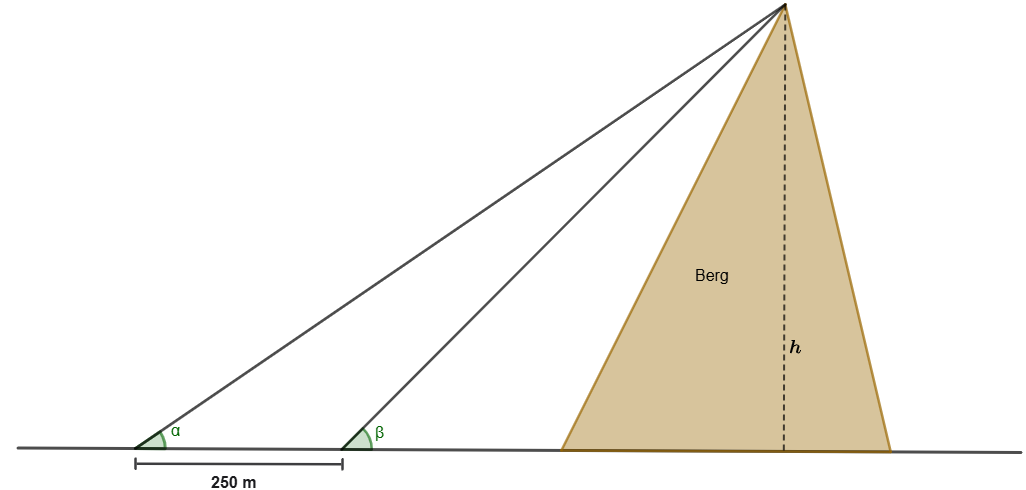
\includegraphics[scale=0.5]{Geometrie/data-geometrie/GZP25_Teil2Aufg4.png}
\end{figure}
\ifthenelse{\boolean{printanswers}}
{\begin{solution}
		\begin{align*}
			\left\{\begin{array}{l} h=\tan{42^\circ}\*(x+250)\\ h=\tan{59^\circ}\*x\end{array}\right.&\Rightarrow\left\{\begin{array}{l} h= 490.43 \\ x=294.68\end{array}\right.
		\end{align*}
\end{solution}}
{\vspace{5pt}\antwort{17}\newpage}


%------------------------------------------------
\question[3]
\begin{minipage}{0.65\linewidth}
	In einer geraden, quadratischen Säule misst die Seite des Grundquadrates $1$ m. Die Körperdiagonale $d=\overline{AD}$ ist um $40\%$ kürzer als der kürzeste Weg, auf dem man von $A$ über $B$ und $C$ nach $D$ gelangen kann.\\ Berechne die Höhe der Säule $h$.
\end{minipage}
\hfill
\begin{minipage}{0.3\linewidth}
	\centering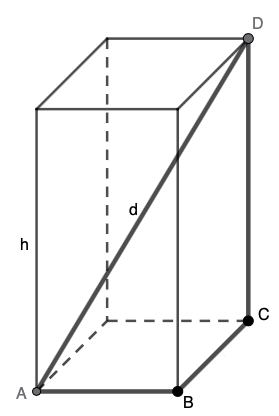
\includegraphics[scale=0.4]{Geometrie/data-geometrie/GZP25_Teil2Aufg6.png}
\end{minipage}
\ifthenelse{\boolean{printanswers}}
{\begin{solution}
		Der Weg über die Kanten ist $1+1+h$.\newline Die Körperdiagonale hat die Länge $\sqrt{1+1+h^2}$.\newline Daraus folgt:
		\begin{align*}
			\sqrt{1+1+h^2}&=(1+1+h)-(1+1+h)\*0.4\\
			\sqrt{1+1+h^2}&=(1+1+h)\*0.6\\
			&\ \\
			&\overset{\text{TR}}{\Rightarrow} h_1=0.5, h_2=1.75
		\end{align*}
\end{solution}}
{\vspace{5pt}\antwort{18.5}\newpage}


%------------------------------------------------
\question[5]
Die Parabel mit der Gleichung $f:y=ax^2+bx+c$ hat den Scheitelpunkt (vertex) $S(-1 \vert 5)$ und schneidet die Gerade $g:y=5x-43$ bei $x=3$. Berechne den zweiten Schnittpunkt (intersection) der Parabel mit der Geraden.
\ifthenelse{\boolean{printanswers}}
{\begin{solution}
		Die $y-$ Koordinate des Schnittpunktes ist: \[y=5\*3-43=-28 \Rightarrow S_1(3,-28).\] Daraus folgt mit der Scheitelpunktform die Funktionsgleichung der Parabel:
		\begin{align*}
			-28&=a(3+1)^2+5 \\
			-33&=a\*16\\
			a&=-\frac{33}{16}\qquad\Rightarrow f:y=-\frac{33}{16}(x+1)^2+5
		\end{align*}
		Wir schneiden nun also die Parabel mit der Gerade:
		\begin{align*}
			-\frac{33}{16}(x+1)^2+5&=5x-43\\
			\overset{\text{TR}}{\Rightarrow} x_2&=-\frac{245}{33}
		\end{align*}
		Daraus folgt der zweite Schnittpunkt $S_2(-\frac{245}{33},-\frac{2644}{33})$
\end{solution}}
{\vspace{5pt}\antwort{23}\newpage}


%------------------------------------------------
\question[4]
\begin{minipage}{0.45\linewidth}
	In einem rechtwinkligen Dreieck mit der Hypotenuse $c=10$ cm unterscheiden sich die Kathetenquadrate um $20$ cm$^2$.\\ Berechne die Höhe $h_c$.
\end{minipage}
\hfill
\begin{minipage}{0.52\linewidth}
	\centering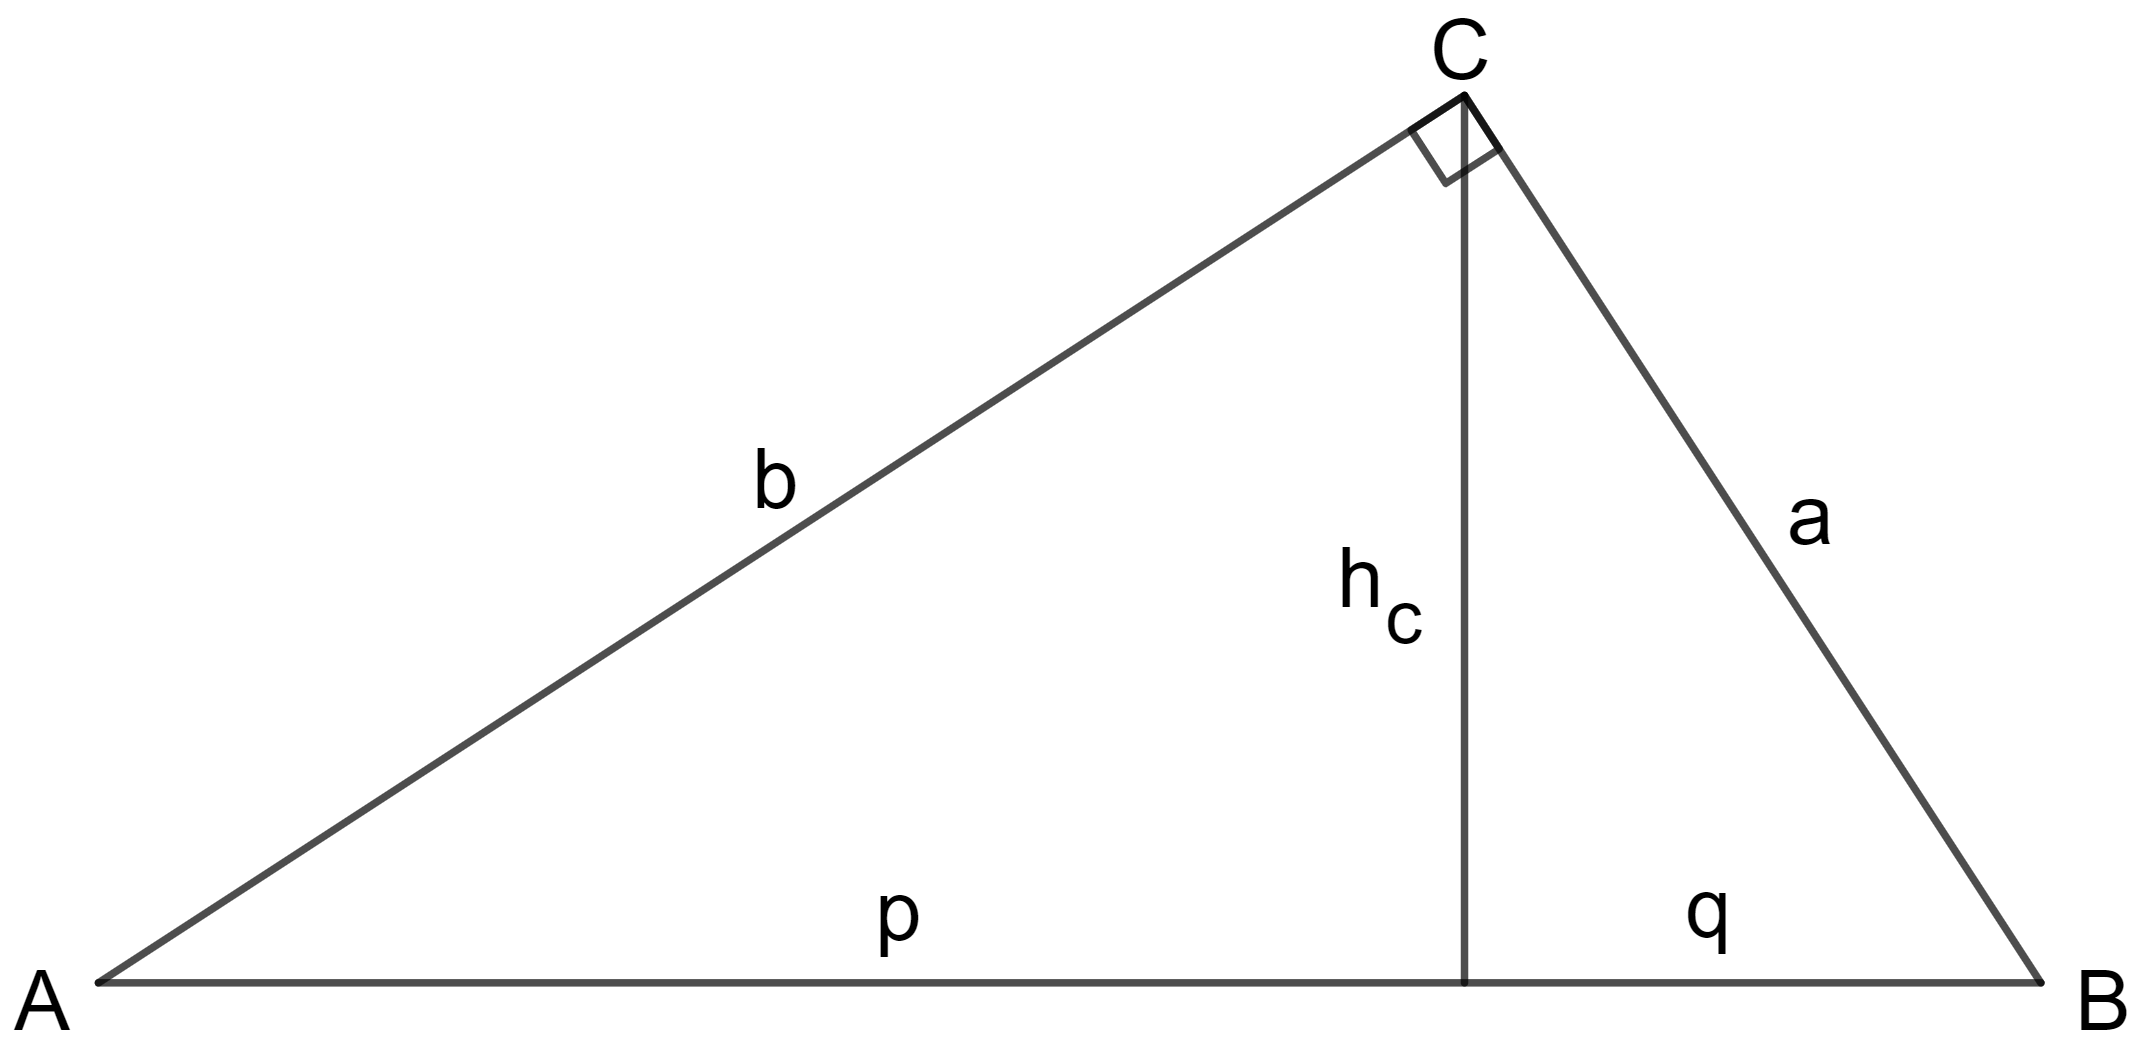
\includegraphics[scale=0.2]{Geometrie/data-geometrie/GZP25_Teil2Aufg2.png}
\end{minipage}
\ifthenelse{\boolean{printanswers}}
{\begin{solution}
		\begin{align*}
			b^2-a^2&=20 && \vert\text{Kathetensatz}\\
			c\*q-c\*p&=20 && \vert\div c\\
			&\systeme{q-p=2,p+q=10}\\
			&\overset{\text{TR}}{\Rightarrow}  p=4, q=6\\
			&\Rightarrow h=\sqrt{p\*q}=\sqrt{24}
		\end{align*}
\end{solution}}
{\vspace{5pt}\antwort{20.5}\newpage}


%------------------------------------------------
\question[4]
Thomas steht gerne früh auf und fährt gerne Velo. Um $06:40$ Uhr startet er jeweils und fährt mit konstanter Geschwindigkeit an die Kanti. Er wohnt $7.5$ km von der Schule entfernt und kommt jeweils um $07:25$ Uhr an. Sein Kollege Franz, der weiter weg wohnt, fährt manchmal mit ihm, aber heute Morgen hat er verschlafen. Franz nimmt deshalb das Töffli, mit dem er konstante $40$ km/h fahren kann, und rast um $07:10$ Uhr am Haus von Thomas vorbei.\newline
Um welche Uhrzeit holt Franz Thomas ein und wie viele Kilometer sind sie dann noch von der Schule entfernt?
\ifthenelse{\boolean{printanswers}}
{\begin{solution}
		Die beiden Bewegungen können mit den folgenden linearen Funktionen beschrieben werden:
		\begin{align*}
			f_{Thomas}:y&=10x\\
			f_{Franz}:y&=40x-20
		\end{align*}
		Schneiden wir die beiden Geraden erhalten wir den Zeitpunkt, wann Franz Thomas einholt:
	\[40x-20=10x \quad\Rightarrow t=\frac{2}{3}h.\]
	Das heisst, sie treffen sich um 07:20 Uhr und sind noch \[7.5-f_{Thomas}\left(\frac{2}{3}\right)=7.5-\frac{20}{3}=0.83km\] von der Schule entfernt.
\end{solution}}
{\vspace{5pt}\antwort{20}}

\ifthenelse{\boolean{printanswers}}
{}{{\bf Reserve:}\newline\antwort{24.5}\newpage{\bf Reserve:}\newline\antwort{24.5}\newpage{\bf Reserve:}\newline\antwort{24.5}}

\endgradingrange{zweiterTeil} % beendet die Unterteilung der Notentabelle
\end{questions}
\end{document}